\documentclass[12pt]{article}

\setlength{\oddsidemargin}{-0.25 in}
\setlength{\evensidemargin}{-0.25 in}
\setlength{\topmargin}{-0.9 in}
\setlength{\textwidth}{7.0 in}
\setlength{\textheight}{9.0 in}
\setlength{\headsep}{0.75 in}
\setlength{\parindent}{0.0 in}
\setlength{\parskip}{0.0 in}

\usepackage{graphicx}
\usepackage{wrapfig}
\usepackage{color}
\usepackage{caption}
\usepackage{subcaption}
\usepackage{longtable}
\usepackage[table]{xcolor}
\usepackage{multirow}

\captionsetup{justification=centering}

\begin{document}
\begin{center}
Analysis of Modified Strassen's Algorithm for Matrix Multiplication \\
Daniel Chen, George Zhang \\
CS124 Programming Assignment 2 Writeup \\
https://github.com/gzhang01/cs124prog/tree/master/prog2 \\
\end{center}

\bigskip

\textbf{Abstract} \\
We implemented a modified version of Strassen's algorithm, where instead of recursing to a base case of a 1 by 1 matrix, we establish a base case of an $n_0$ by $n_0$ matrix and compute the product using standard matrix multiplication at that point. Our goal was to examine the runtime of this modified algorithm in order to determine the best threshold $n_0$. Analytically, we found that the optimal $n_0$ assuming constant time basic operations (addition, subtraction, multiplication, etc.) was about 9-15. Experimentally, we saw that a threshold of 30-50 produced the optimal run time. \\

\textbf{Introduction} \\
The standard matrix multiplication algorithm most people learn requires computing each cell of the product matrix by taking the dot product of the corresponding row / column of the input matrices. This is a $O(n^3)$ algorithm, since it takes $n$ steps to compute each of $n^2$ cells. Strassen's algorithm uses a divide and conquer strategy that requires only $7$ multiplications of matrices of size $n/2$, which results in a $O(n^{\log_2 7}) \approx O(n^{2.81})$ algorithm. Asymptotically, Strassen's algorithm is an improvement over the conventional method. However, for small $n$, the conventional method is faster. \\

Our task was to analyze a modified version of Strassen's algorithm, where instead of recursing to a 1 by 1 matrix, we use a base case of an $n_0$ by $n_0$ matrix and compute the product using conventional matrix multiplication. We wanted to find the threshold $n_0$ that would optimize this algorithm. We also wanted to compare the performances of these three algorithms--conventional multiplication, Strassen's, and our modified Strassen's--to see which performs best for matrices of different sizes. To determine this threshold, we will start by calculating it analytically assuming constant cost of arithmetic operations (addition, subtraction, multiplication, and division of real numbers) and no cost for all other operations. \\

We start by looking at Strassen's algorithm itself. Below is a summary of the operations needed to compute a matrix product using Strassen's, where A through H represent the matrices' quadrants. \\

\begin{table}[h!]
\centering
{\setlength{\tabcolsep}{15pt}
\begin{tabular}{ c c c | c c c }
Variable & Expression &&& Variable & Expression\\ \hline
$P_1$ & $A(F-H)$ &&& $Q_1$ & $P_5+P_4-P_2+P_6$ \\
$P_2$ & $(A+B)H$ &&& $Q_2$ & $P_1+P_2$ \\
$P_3$ & $(C+D)E$ &&& $Q_3$ & $P_3+P_4$ \\
$P_4$ & $D(G-E)$ &&& $Q_4$ & $P_5+P_1-P_3-P_7$ \\
$P_5$ & $(A+D)(E+H)$ & \\
$P_6$ & $(B-D)(G+H)$ & \\
$P_7$ & $(A-C)(E+F)$ & \\
\end{tabular}}
\caption{Summary of Strassen's Algorithm
\label{T:Stra}}
\end{table}

We can see that for a given matrix of dimension $n$, we require 7 multiplications of matrices of dimension $n/2$. In addition, there are 18 additions/subtractions of matrices of size $n/2$, which contain $(n/2)^2$ elements. Thus we can write a recurrence equation describing the run time of standard Strassen's:
$$f(n) = 7f\left(\frac{n}{2}\right)+18\left(\frac{n}{2}\right)^2$$
$$f(1) = 1$$

For conventional matrix multiplication, where we compute the dot product of rows and columns, we have a total of $n^3$ multiplications and $n^2(n - 1)$ additions. As a result, the run time for this algorithm can be expressed in closed form easily:
$$s(n) = n^2(2n-1)$$

Our modified algorithm will combine these two procedures. We know that if $n > n_0$, then we perform Strassen's. If $n < n_0$, we have reached our base case and we perform standard matrix multiplication. Thus our recurrence equation is:
$$f(n) = 7f\left(\frac{n}{2}\right)+18\left(\frac{n}{2}\right)^2, n > n_0$$
$$f(n) = s(n), n \le n_0$$

This recurrence is difficult to solve. Let us simply solve it numerically by looking at $f(n)$ for various values of $n$ and $n_0$:

\begin{table}[h!]
\centering
\renewcommand{\arraystretch}{1.2}
{\setlength{\tabcolsep}{5pt}
\begin{tabular}{c|c|c|c|c|c|c|c|c}
\multirow{2}{*}{$n_0$} & \multicolumn{5}{c}{$n$}\\ \cline{2-9}
& 2 & 4 & 8 & 16 & 32 & 64 & 128 & 256 \\ \hline
3 & \cellcolor{green}12 & 156 & 1,380 & 10,812 & 80,292 & 580,476 & 4,137,060 & 29,254,332 \\
6 & \cellcolor{green}12 & \cellcolor{green}112 & 1,072 & 8,656 & 65,200 & 474,832 & 3,397,552 & 24,077,776 \\
9 & \cellcolor{green}12 & \cellcolor{green}112 & \cellcolor{green}960 & \cellcolor{green}7,872 & \cellcolor{green}59,712 & \cellcolor{green}436,416 & \cellcolor{green}3,128,640 & \cellcolor{green}22,195,392 \\
12 & \cellcolor{green}12 & \cellcolor{green}112 & \cellcolor{green}960 & \cellcolor{green}7,872 & \cellcolor{green}59,712 & \cellcolor{green}436,416 & \cellcolor{green}3,128,640 & \cellcolor{green}22,195,392 \\
15 & \cellcolor{green}12 & \cellcolor{green}112 & \cellcolor{green}960 & \cellcolor{green}7,872 & \cellcolor{green}59,712 & \cellcolor{green}436,416 & \cellcolor{green}3,128,640 & \cellcolor{green}22,195,392 \\
18 & \cellcolor{green}12 & \cellcolor{green}112 & \cellcolor{green}960 & 7,936 & 60,160 & 439,552 & 3,150,592 & 22,349,056 \\
21 & \cellcolor{green}12 & \cellcolor{green}112 & \cellcolor{green}960 & 7,936 & 60,160 & 439,552 & 3,150,592 & 22,349,056 \\
24 & \cellcolor{green}12 & \cellcolor{green}112 & \cellcolor{green}960 & 7,936 & 60,160 & 439,552 & 3,150,592 & 22,349,056 \\
\end{tabular}}
\caption{Theoretical Run Time of Modified Strassen's}
\end{table}

We can see from this analysis that the optimal threshold is around 9-15, as the number of operations we need to do is minimal for these thresholds as $n$ increases. \\

\bigskip

\pagebreak

\textbf{Implementation} \\
We also attempted to find the threshold experimentally by implementing our modified Strassen's algorithm. To start, we created a new matrix type to encapsulate the information we would need. This type includes a 2D array of ints (representing the matrix itself), the dimension of the matrix, and the start row and start column, which are used to avoid copying large amounts of data when splitting matrices in Strassen's algorithm. In addition, we created basic functions to create a matrix, free the matrix, get / set elements, get the rows / columns, and add matrices (see matrix.c). We also included a function to pretty print the matrix to simplify debugging. \\

We then moved on to implementing conventional matrix multiplication (see matrixMultiplication.c). This process was also relatively straightforward. Using three nested for loops, we can iterate through all the necessary sums and products to calculate the matrix product. From prior knowledge of caching behavior, we used a column-first method that runs slightly faster than the standard dot product method. This speedup is due to the fact that we have more cache hits in the former than the latter, so we touch memory less frequently, which speeds up our algorithm. \\

Implementing Strassen's algorithm was a bit more technical. We wrote a function to split a given matrix into four matrices of size $n/2$ (see matrix.c). With our matrix type, this was relatively simple, as we could just point to the same array of numbers but assign different start rows and columns. After splitting, we simply implemented the various additions and multiplications necessary to produce the quadrants we want in our product matrix. Finally, we populated the product matrix quadrant by quadrant, again by taking advantage of the start column and row variables. Our modified Strassen's algorithm simply changed the base case of Strassen's to use the $n_0$ by $n_0$ base case instead of the 1 by 1 case. \\

However, this approach would only work if we did not run into a matrix with odd dimensionality while splitting our matrices. To resolve this issue, we added some padding to our matrix to begin with, so that we would never have to split a matrix with odd dimensions. Instead of simply padding to the next power of two, which we realized would be expensive for large $n$, we realized that once we hit our threshold and started performing conventional matrix multiplication, the dimensions of our matrix no longer mattered. Thus our padding function divided our dimension in half (taking the ceiling if necessary) until we were below our threshold and then multiplied back up to ensure that we could divide evenly when splitting our matrix. \\

With these functions written, we proceeded to collect data by running our algorithm on various dimensions and thresholds. We were particularly interested in how changes in threshold affect runtime, but we also wanted to see whether the dimensionality of the matrix affected the threshold. \\

\bigskip

\textbf{Testing} \\
We evaluated our algorithm by inputting matrices with known results, using the identity matrix for example. Once we verified the correctness of our conventional matrix multiplication, we could also use it to check that our Strassen's implementation was correct by comparing the output of solely the conventional matrix multiplication function against the result of the Strassen's algorithm.

\pagebreak

\textbf{Results} \\
We ran and timed our program on matrices of dimension $600$, $800$, $1000$, and $1200$ with threshold values ranging from $5$ to $395$ at interval $5$. The entire data set is available in appendix A. Below, we have reproduced the data at intervals of $10$ up until $150$. Note that for each threshold-dimension pair, the run time is calculated from the average of 5 runs, and all run times are given in seconds.

\begin{table}[h]
\centering
{\setlength{\tabcolsep}{15pt}
\begin{tabular}{c|c|c|c|c}
threshold & d = 600 & d = 800 & d = 1000 & d = 1200 \\\hline
10 & 12.4 & 35.0 & 48.4 & 84.4 \\
20 & 10.0 & 24.8 & 43.2 & 68.0 \\
30 & 10.0 & 21.4 & 43.0 & 68.0 \\
40 & 10.0 & 21.6 & 43.4 & 69.4 \\
50 & 10.0 & 22.6 & 43.4 & 69.0 \\
60 & 10.2 & 22.2 & 43.0 & 69.0 \\
70 & 10.2 & 22.2 & 43.8 & 69.0 \\
80 & 10.4 & 22.0 & 44.0 & 72.0 \\
90 & 10.6 & 22.6 & 44.0 & 71.6 \\
100 & 10.6 & 24.6 & 44.0 & 71.6 \\
110 & 10.4 & 24.6 & 44.0 & 71.4 \\
120 & 10.2 & 24.4 & 43.8 & 71.2 \\
130 & 10.6 & 24.4 & 47.2 & 71.4 \\
140 & 10.4 & 24.6 & 47.4 & 71.4 \\
150 & 11.6 & 24.4 & 47.6 & 79.2 \\
\end{tabular}}
\caption{Run Times of Modified Strassen's for Various Thresholds and Dimensions}
\end{table}

The trend is difficult to see in a table, but it appears that the low run times appear to be with a threshold of around 20-60. We also plotted all our data on graphs to better visualize the trends (see Figure \ref{results} on next page). \\

\begin{figure}
\centering
\begin{subfigure}{.5\textwidth}
  \centering
  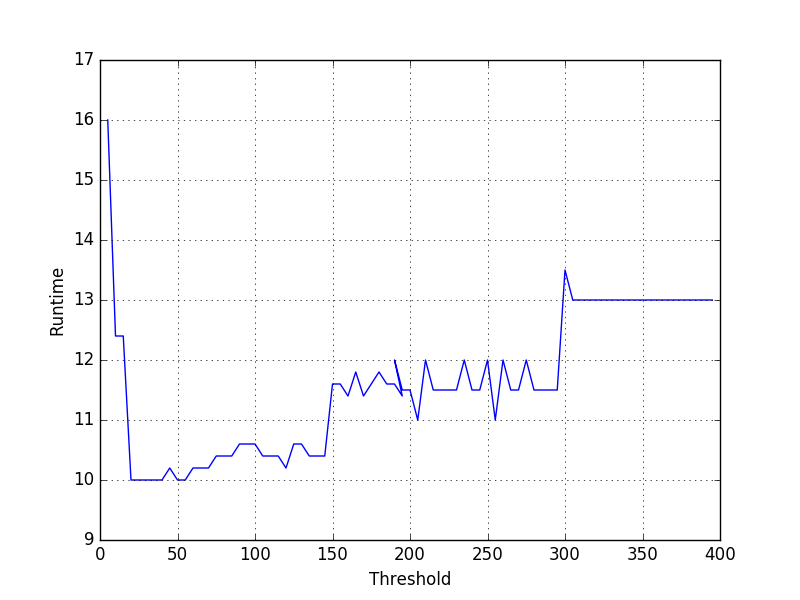
\includegraphics[width=\linewidth]{data/d600.png}
  \caption{Run Time vs. Threshold (dim $= 600$)}
  \label{fig:sub1}
\end{subfigure}%
\begin{subfigure}{.5\textwidth}
  \centering
  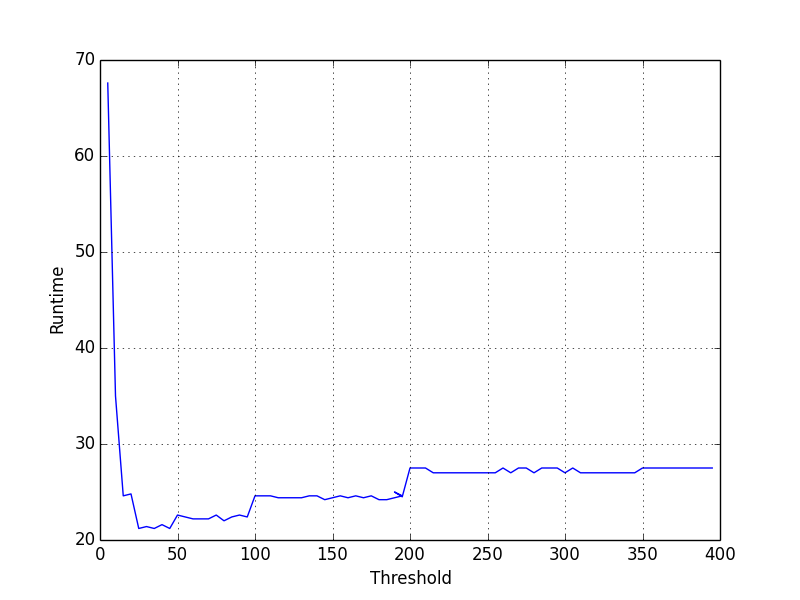
\includegraphics[width=\linewidth]{data/d800.png}
  \caption{Run Time vs. Threshold (dim $= 800$)}
  \label{fig:sub2}
\end{subfigure} \\ % 
\bigskip
\begin{subfigure}{.5\textwidth}
  \centering
  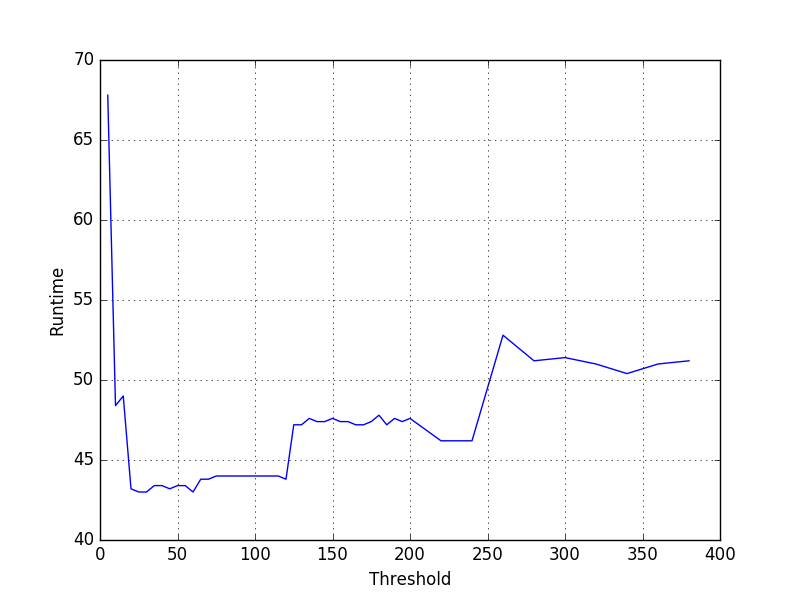
\includegraphics[width=\linewidth]{data/d1000.png}
  \caption{Run Time vs. Threshold (dim $= 1000$)}
  \label{fig:sub3}
\end{subfigure}%
\begin{subfigure}{.5\textwidth}
  \centering
  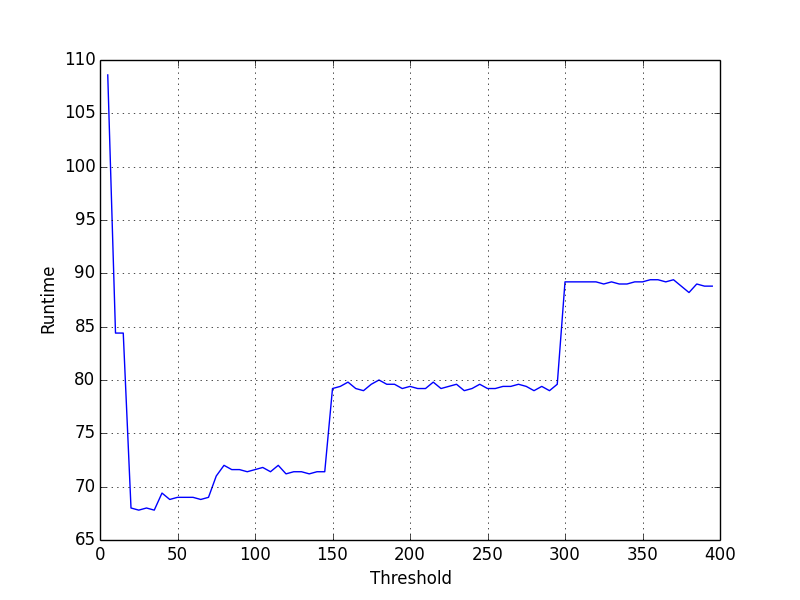
\includegraphics[width=\linewidth]{data/d1200.png}
  \caption{Run Time vs. Threshold (dim $= 1200$)}
  \label{fig:sub4}
\end{subfigure}%
\caption{Plots of Results}
\label{results}
\end{figure}

From these plots, we can see that the run times do in fact dip early on, roughly around 20-60 for dimension 600 and 1000 matrices, about 20-45 for dimension 800, and about 20-40 for dimension 1200. Since these times only came from the average of 5 runs, and since run time measurements are inherently slightly variable (resource allocation may easily produce noisy results) we are unable to provide a specific numerical threshold. However, the range 30-50 appears to be roughly optimal for each of these test cases. Much lower or higher than this results in significantly higher run times. \\

We also decided to investigate how our modified Strassen's algorithm compared to standard Strassen's (with base case 1 by 1) and conventional matrix multiplication. The results are shown in Table \ref{table:comp} on the next page. Note that each of these were run only once, the threshold used for modified Strassen's was 40, and standard Strassen's was not run for dim = 800, 1000. \\

\begin{table}
\centering
{\setlength{\tabcolsep}{10pt}
\begin{tabular}{c|c|c|c}
dimension & conventional & standard Strassen's & modified Strassen's \\\hline
200 & \cellcolor{green}1 & 8 & \cellcolor{green}1 \\
400 & 4 & 56 & \cellcolor{green}3 \\
600 & 15 & 398 & \cellcolor{green}10 \\
800 & 35 & --- & \cellcolor{green}21 \\
1000 & 67 & --- & \cellcolor{green}43 \\
\end{tabular}}
\caption{Comparison of Matrix Multiplication Algorithms}
\label{table:comp}
\end{table}

As we can see, our modified Strassen's algorithm runs faster than the conventional algorithm and the standard Strassen's algorithm when $n$ is large. \\

\bigskip

\pagebreak

\textbf{Discussion} \\
Our goal was to implement and find the threshold for our modified Strassen's algorithm. Analytically, we rewrote the recurrence equation for our modified algorithm and using dynamic programming, we wrote a script to calculate the number of operations needed to find the matrix product given different dimensions and thresholds. Using this method, we found the cutoff to be around 9-15. Experimentally, we implemented our modified algorithm and tested with various dimensions and values for thresholds. We found that a threshold of about 30-50 was optimal for our implementation. \\

We need to consider why there is this discrepancy between our analytical result and our experimental result. First, our analytical result assumed certain costs that may not be consistent with what is true in an experimental setting. For example, we assumed that non-arithmetic operations were free. However, in our implementation, we needed to allocated memory in order to create our matrices. Allocating memory is definitely not a free operation, even though our analytical analysis assumed it was. As a result, we would expect the Strassen's part of our algorithm to take longer experimentally than we would predict given our assumptions. This longer run time would encourage us to switch over to conventional matrix multiplication sooner in our calculations, which is analogous to a higher threshold. \\

Along the same lines, our arithmetic operations may not have cost 1. In reality, calculating basic arithmetic processes would require getting the numbers, which may need to touch memory if not in the cache, perform the operation, and assign the resulting value to some variable. Especially if we have a cache miss, this operation may not always have the same cost. As a result, we would again expect the actual run time to be slower than our prediction, and so we would have a higher threshold. \\

Our calculations were done with matrices of relatively high dimensions. We made this choice because we wanted several iterations of Strassen's before we reached our base case. If we ran with a low-dimension matrix, such as dim $= 100$, then we would not see as much variation in the run times. Indeed, we collected some data for dim $= 400$ and saw that the run times were generally not that different for various thresholds, and so we decided to use larger matrices to more effectively show the effects of the threshold on run time. \\

Finally, we want to address the behavior of the graphs that we produced from our results. Because of the way we implemented our padding, the amount of padding needed does not strictly increase as the threshold increases. Therefore, given increasing dimensionality, the dimensions of the matrices we actually work with in our algorithm are not strictly increasing. In addition, even in areas where it is strictly increasing, it does not necessarily increase linearly. Because of the variable sizes of the matrices we actually work with, we expect run time to increase in the long run, but we also expect local variability. This is indeed what we see in our graphs.


\pagebreak
\begin{table}[h]
\centering
\caption*{\textbf{Appendix A}: Run Times of Modified Strassen's for Various Thresholds and Dimensions}
{\setlength{\tabcolsep}{15pt}
\begin{longtable}{c|c|c|c|c}
threshold & d = 600 & d = 800 & d = 1000 & d = 1200 \\\hline
5 & 16.0 & 67.6 & 67.8 & 108.6\\
10 & 12.4 & 35.0 & 48.4 & 84.4\\
15 & 12.4 & 24.6 & 49.0 & 84.4\\
20 & 10.0 & 24.8 & 43.2 & 68.0\\
25 & 10.0 & 21.2 & 43.0 & 67.8\\
30 & 10.0 & 21.4 & 43.0 & 68.0\\
35 & 10.0 & 21.2 & 43.4 & 67.8\\
40 & 10.0 & 21.6 & 43.4 & 69.4\\
45 & 10.2 & 21.2 & 43.2 & 68.8\\
50 & 10.0 & 22.6 & 43.4 & 69.0\\
55 & 10.0 & 22.4 & 43.4 & 69.0\\
60 & 10.2 & 22.2 & 43.0 & 69.0\\
65 & 10.2 & 22.2 & 43.8 & 68.8\\
70 & 10.2 & 22.2 & 43.8 & 69.0\\
75 & 10.4 & 22.6 & 44.0 & 71.0\\
80 & 10.4 & 22.0 & 44.0 & 72.0\\
85 & 10.4 & 22.4 & 44.0 & 71.6\\
90 & 10.6 & 22.6 & 44.0 & 71.6\\
95 & 10.6 & 22.4 & 44.0 & 71.4\\
100 & 10.6 & 24.6 & 44.0 & 71.6\\
105 & 10.4 & 24.6 & 44.0 & 71.8\\
110 & 10.4 & 24.6 & 44.0 & 71.4\\
115 & 10.4 & 24.4 & 44.0 & 72.0\\
120 & 10.2 & 24.4 & 43.8 & 71.2\\
125 & 10.6 & 24.4 & 47.2 & 71.4\\
130 & 10.6 & 24.4 & 47.2 & 71.4\\
135 & 10.4 & 24.6 & 47.6 & 71.2\\
140 & 10.4 & 24.6 & 47.4 & 71.4\\
145 & 10.4 & 24.2 & 47.4 & 71.4\\
150 & 11.6 & 24.4 & 47.6 & 79.2\\
155 & 11.6 & 24.6 & 47.4 & 79.4\\
160 & 11.4 & 24.4 & 47.4 & 79.8\\
165 & 11.8 & 24.6 & 47.2 & 79.2\\
170 & 11.4 & 24.4 & 47.2 & 79.0\\
175 & 11.6 & 24.6 & 47.4 & 79.6\\
180 & 11.8 & 24.2 & 47.8 & 80.0\\
185 & 11.6 & 24.2 & 47.2 & 79.6\\
190 & 11.6 & 24.4 & 47.6 & 79.6\\
195 & 11.4 & 24.6 & 47.4 & 79.2\\
\end{longtable}}
\end{table}
\begin{table}[h]
\centering
{\setlength{\tabcolsep}{15pt}
\begin{longtable}{c|c|c|c|c}
threshold & d = 600 & d = 800 & d = 1000 & d = 1200 \\\hline
200 & 12.0 & 28.0 & 47.2 & 79.4\\
205 & 12.0 & 27.6 & 46.6 & 79.2\\
210 & 12.0 & 28.2 & 46.0 & 79.2\\
215 & 12.0 & 27.6 & 46.2 & 79.8\\
220 & 12.0 & 27.8 & 46.0 & 79.2\\
225 & 12.0 & 27.4 & 46.0 & 79.4\\
230 & 11.6 & 27.8 & 46.2 & 79.6\\
235 & 12.0 & 27.8 & 46.0 & 79.0\\
240 & 12.0 & 28.0 & 46.0 & 79.2\\
245 & 11.8 & 27.8 & 46.4 & 79.6\\
250 & 11.8 & 27.2 & 51.8 & 79.2\\
255 & 12.0 & 27.8 & 51.8 & 79.2\\
260 & 12.0 & 27.4 & 51.4 & 79.4\\
265 & 12.4 & 27.8 & 51.8 & 79.4\\
270 & 12.0 & 27.6 & 51.4 & 79.6\\
275 & 11.8 & 28.0 & 51.8 & 79.4\\
280 & 11.6 & 28.2 & 51.6 & 79.0\\
285 & 12.0 & 28.2 & 51.6 & 79.4\\
290 & 12.0 & 27.8 & 51.8 & 79.0\\
295 & 12.0 & 28.6 & 51.8 & 79.6\\
300 & 13.2 & 27.8 & 51.8 & 89.2\\
305 & 13.4 & 27.4 & 51.4 & 89.2\\
310 & 13.6 & 27.8 & 51.6 & 89.2\\
315 & 13.2 & 27.8 & 52.0 & 89.2\\
320 & 13.2 & 27.6 & 51.6 & 89.2\\
325 & 13.4 & 28.0 & 51.2 & 89.0\\
330 & 13.2 & 28.0 & 52.0 & 89.2\\
335 & 13.4 & 27.8 & 51.4 & 89.0\\
340 & 13.0 & 27.8 & 51.6 & 89.0\\
345 & 13.2 & 27.8 & 51.6 & 89.2\\
350 & 13.6 & 27.8 & 51.6 & 89.2\\
355 & 13.4 & 28.0 & 51.6 & 89.4\\
360 & 13.4 & 27.8 & 51.8 & 89.4\\
365 & 13.4 & 28.0 & 51.6 & 89.2\\
370 & 13.2 & 28.0 & 51.8 & 89.4\\
375 & 13.6 & 27.4 & 51.6 & 88.8\\
380 & 13.2 & 27.6 & 51.4 & 88.2\\
385 & 13.2 & 27.6 & 51.6 & 89.0\\
390 & 13.4 & 28.4 & 51.8 & 88.8\\
395 & 13.4 & 28.6 & 51.6 & 88.8\\
\end{longtable}}
\end{table}


\end{document}








